\SSbreak\\
\emph{Source: Unknown}\\
\emph{Proposer: \Pchris}\\ %\Pchan \Pbrain \Pss
\emph{Problem ID: 201}\\
\emph{Date: 2021-05-22}\\
\emph{Difficulty: Challenging}\\
\SSbreak
 
\SSpsetQ{
    $\triangle ABC$ has circumcircle $\Gamma$ and incentre $I$, with sidelengths $AB = 44, BC = 37, CA = 15$. Let $L$ be the midpoint of the arc $\widehat{BC}$ containing $A$. 
    $\overleftrightarrow{LI}$ meets $\Gamma$ again at $D$, and the tangent to $\Gamma$ at $A$ meets $\overleftrightarrow{BC}$ at $P$.
    $\overleftrightarrow{PD}$ meets $\Gamma$ again at $X$. If $Y$ is the point on $\overline{BC}$ such that $\angle BAX = \angle CAY$,
    the ratio $\frac{BY}{CY}$ can be expressed in the form $\frac{m}{n},$ where $m, n$ are relatively prime positive integers. Find $100m + n$.
    %Put Problem Here
}\bigskip

\begin{solution}\hfil\medskip

    \begin{center}
        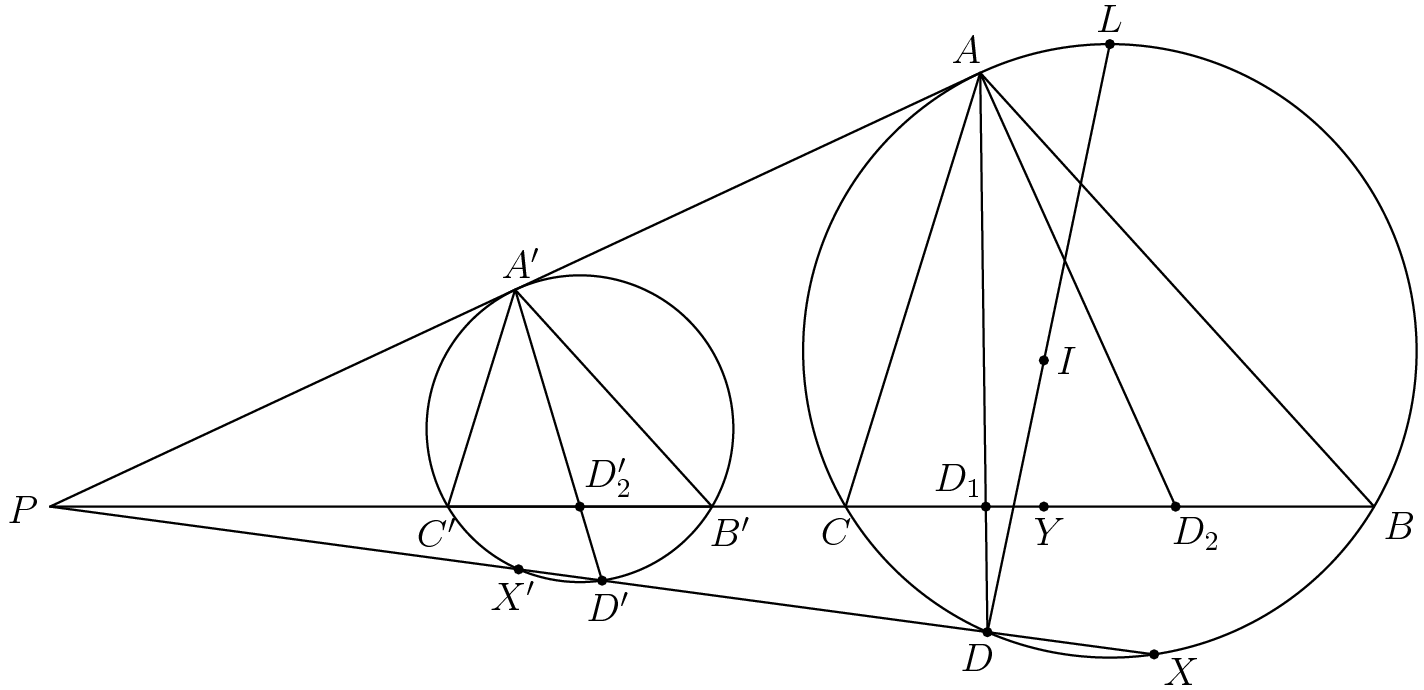
\includegraphics[scale=0.4]{Sections/Files/14-2-6.png}
    \end{center}
	
    We claim that for a general cevian $\ell$ through $A$, $Y$ will be the reflection across the midpoint $M$ of $\overline{BC}$ of the intersection of the isogonal
    line of $\ell$ and $\overline{BC}$. Consider the following transformation that sends points on $\overline{BC}$ to points on $\overline{BC}$: take the projections of points
    wrt $A$ onto $\Gamma$, invert $\triangle ABC$ and those points wrt $P$, project points back onto $\overline{BC}$ wrt $A$, then invert the points back onto the original $\triangle ABC$.
    Let $\overline{AD}$ intersect $\overline{BC}$ at $D_1$, and let $D_2$ be the intersection of the isogonal line of $\overline{AD}$ and $\overline{BC}$. Applying
    this transformation to $\overline{AD}$ and $\overline{AX}$, we let $D', X', B', C', D_2'$ be the images of $D, X, B, C, D_2$ under inversion, and $Y'$ the intersection of $\overline{AD'}$
    and $\overline{B'C'}$; by angle chase we have $\overline{AX'}$ isogonal to $\overline{AD}$ and $\overline{AD'}$ isogonal to $\overline{AX}$. 
    By inversion distance formula we find $$\frac{BY}{CY} = \frac{CD_2}{BD_2} = \frac{PB}{PC};$$ furthermore since $\overline{PA}$ is a tangent 
    we have $\overline{A'C'} \parallel \overline{AB}, \overline{A'B'} \parallel \overline{AC}$ and $\overline{AD'} \parallel \overline{AX}, \overline{AX'} \parallel \overline{AD}$
    so by similar triangles and inversion distance formula we have $$\dfrac{C'D_2'}{A'D_2'} = \dfrac{BD_1}{AD_1}, \dfrac{B'D_2'}{A'D_2'} = \dfrac{CD_1}{AD_1} \iff \dfrac{C'D_2'}{B'D_2'} = \dfrac{PB}{PC} = \dfrac{BD_1}{AD_1} = \dfrac{CD_2}{BD_2}$$
    and we are done. \medskip

    In the case of this problem, it is well-known (in EGMO; invert at A) that $D$ is the touchpoint of the $A$-mixtilinear incircle and $\Gamma$, and so the isogonal line pases through
    the $A$-excircle touchpoint, so $Y$ is actually the incircle touchpoint on $\overline{BC}$ so our answer is $\frac{s - b}{s - c} = \frac{33}{4} \iff \boxed{3304}.$
    %Put sol here
\end{solution}\bigskip
